\documentclass[]{article}
%\documentclass[]{../../../../tex/classes/homework}
\usepackage{../../../../tex/packages/hebrewSupport}
\usepackage{../../../../tex/packages/mathShortcuts}
%\usepackage{../../../../tex/packages/theoremsSupport}

\usepackage{pgfplots}
\usepgfplotslibrary{fillbetween}
\usepackage{nicematrix}

\usepackage{multicol}


%% Math packages
\RequirePackage{ifxetex,ifluatex,amssymb,amsmath,mathrsfs,amsthm,witharrows,mathtools,mathdots,centernot}
\RequirePackage{amsmath}
\renewcommand{\qedsymbol}{$\blacksquare$} % end proofs with \blacksquare. Overwrites the defualts.
\RequirePackage{bm}

% Design
\RequirePackage[margin=1in]{geometry}
\RequirePackage[skip=4pt, indent=0pt]{parskip}
\RequirePackage[normalem]{ulem}
\renewcommand\labelitemi{$\bullet$}


\newcommand\ff{\mathrm{f}}
\newcommand\gcc{G^{\mathrm{SCC}}}
\newcommand\squigT{\overset{T}{\squig}}
\newcommand\squigd{\leftrightsquigarrow}
\DeclareMathOperator{\low}{low}
\DeclareMathOperator{\sol}{sol}
\DeclareMathOperator{\val}{val}
\DeclareMathOperator{\key}{key}
\DeclareMathOperator{\Left}{left}
\DeclareMathOperator{\Right}{right}

\setlength{\parindent}{0pt}
\setlength{\parskip}{4pt}



\DeclareMathOperator*{\argmin}{arg\,min}
\newcommand\I  {(\mathrm{I})}
\newcommand\II {(\mathrm{II})}

\newcommand\qq  {(\mathrm{1})}
\newcommand\ww  {(\mathrm{2})}
\newcommand\ee  {(\mathrm{3})}
\newcommand\rr  {(\mathrm{4})}
\newcommand\str {^{\star}}

\author{שחר פרץ}
\title{אלגוריתמים $\sim$ \textit{תרגיל בית 5}}
\begin{document}
%	\maketitle
	
	\ {} \\ \ \\ \ \\ 
%	\section{}

	תהא $G = (V, E, c, s, t)$ רשת זרימה עם $c \co E \to \Z$ וזרימה מקסימלית $f \co E \to \Z_{\ge 0}$. תהי $e^\star \in E$. 
	\begin{enumerate}
		\item נוכיח שאם $f(e\str) > 0$ אז $e\str$ על מעגל שבו כל הקשתות בעלות זרימה חיובית, או שהיא על מסלול מ־$s$ ל־$t$. 
		\begin{proof}
			נתאר אלגוריתם שמוצא מעגל או מסלול כזה. נגדיר ב־$\tl E$ את הצמצום של $G$ על הקשתות עם זרם חיובי ב־$f$. נסמן $e\str = (u, v)$
			\begin{itemize}
				\item נריץ DFS על $\tl G$ מ־$v$. אם מצאנו מעגל נחזיר אותו, אחרת מצאנו מסלול ל־$t$. 
				\item נריץ DFS על $\tl G^T$ מ־$u$. אם מצאנו מעגל נחזיר אותו, אחרת מצאנו מסלול ל־$s$. 
			\end{itemize}
			לבסוף אם לא מצאנו מעגלים נחזיר את $s \squig v \to u \squig t$ שמצאנו. 
			
			נפנה להוכיח את נכונות האלגוריתם. ברור שאם מצאנו מסלול הוא חיובי (שכן הוא ב־$\tl G$) ואז סיימנו. אך כאורה לא מובטח לנו ש־DFS יוכל להמשיך לנצח עד הגעה ל־$t$ או $s$, או עד למציאת מעגל: אך בהנחה ש־DFS עבר בדיוק על $(w_1, w_2)$ כלשהי, בהכרח $f(w_1, w_2) > 0$ ולכן מאילוץ הקיבול סכום הזרימות היוצאות $\sum_{\tl v \in V} f(w_1, \tl v) > 0$ דהיינו יש קשת חיובית כלשהי שיוצאת מ־$(w_1, w_2)$ וה־DFS יוכל להמשיך להתקדם (אלא אם זו קשת שהוא כבר גילה, ואז סגרנו מעגל). באופן זהה בעבור הגרף המשוחלף (רק הפוך, הסכום $\sum_{\tl v \in V} f(\tl v, w_1)$ יהיה חיובי). משום שה־DFS תמיד יוכל להתקדם, האלגוריתם שתיארנו אכן יסתיים במציאת מעגל או במסלול $s \squig t$ דרך $e \str = (v, u)$ בהכרח. 
		\end{proof}
		\textit{הערה: }הסיבוכיות של הרצת שני DFS־ים ובניית גרף משוחלף היא $\oc(\sof + \sof E)$. 
		\item נניח שהקיבול של $e\str$ גדל ב־$1$. נמצא באופן יעיל זרימת מקסימום. 
		\begin{itemize}
			\item \textbf{אלגוריתם: }נבדוק האם $e\str$ הייתה רוויה ב־$f$ לפני ההעלאה. אם זה לא המצב, הרצה של איטרצית FF יחידה עליו תוכל להחזיר זרימה מגודל $\sof f + 1$, ולכן מקסימלית. אם זה כן המצב, נחזיר את $f$ כמו שהיא. 
			\item \textbf{נכונות: }אם $e\str$ אינה רוויה, העלאה של קיבולה לא משנה בכל מקרה. אחרת, ב־$E_f$ המקורי אין כלל מסלול $s \squig t$, ומשום שעתה הוספנו קשת יחידה (עם קיבול $1$) על $e\str$, מסלול משפר של FF בהכרח יעבור דרכה. אם שיפור לאורך מסלול שמשתמש ב־$e\str$ לא מוביל לעלייה בערך הזרימה, אף מסלול אחר לא יצליח לעשות זאת (אחרת זו סתירה למקסימליות $f$). אם הצלחנו לשפר, אז מצאנו זרימה מגודל $\sof f + 1$, שזה המקסימום שנוכל למצוא בגרף זה (כי העלנו רק קיבול אחד ב־$1$). 
			\item \textbf{סיבוכיות: }עלות הרצת FF לאיטרציה יחידה יעלה $\oc(\sof V + \sof E)$. 
		\end{itemize}
		\item נניח שהקיבול של $e\str$ קטן ב־$1$. נמצא באופן יעיל זרימת מקסימום. 
		\begin{itemize}
			\item \textbf{אלגוריתם: }גם כאן נבדוק האם $e\str$ הייתה רוויה. אם היא לא הייתה רוויה, נוכל להחזיר את הזרימה $f$ שהתחלנו ממנה. אחרת נמצא מסלול שעובר דרך $e\str$, נחסיר לאורכו $1$ (כדי לקבל זרימה תקינה) ונריץ EK עליו. נחזיר את הזרימה שתתקבל. 
			\item \textbf{נכונות: }לפני שהסרנו $-1$ לאורך המסלול הכולל את $e\str$, לא היה מסלול $s \squig t$. נבחין ש־$f$ לאחר חיסור של $-1$ לאורך מסלול בה זרימה תקינה (חיבור/חיסור של מסלול אחר), ולאחר איטרציה של EK בהכרח שוב $t$ לא יהיה נגיש מ־$s$ (שכן EK עומד להשתמש בקשת כלשהי במסלול היחידי בין $s$ ל־$t$ בגרף השיורי). סה''כ בסוף האיטרציה הגענו לגרף שיורי בו $t$ לא נגיש מ־$s$ ולכן מדובר בזרימת מקסימום. 
			
			(הערה: אם האלגוריתם מצא מעגל שעליו $e\str$ נמצאת, אז גם לאחר חיסור $-1$־ים מהמעגל וקבלת זרימה תקינה, נבחין שהגרף השיורי ללא מסלול משפר כלשהו, וגם כאן נעצור ונוכל להחזיר את הזרימה)
			\item \textbf{סיבוכיות: }עלות האלגוריתם מהסעיף א' יעלה $\oc(\sof V + \sof E)$. עלות איטרציה אחת של EK תהיה $\oc(\sof V + \sof E)$, וסה''כ סיבוכיות לינארית. 
		\end{itemize}
	\end{enumerate}
	
		\newpage \ \newpage 
%	\npage
%	\section{}
	תהא רשת זרימה. 
	\begin{enumerate}[(A)]
		\item נדגים זרימה שמוחזרת מ־FF שבה יש מעגל שעל קשתותיו זרימה חיובית. נתבונן בגרף $V = \{s, t\}, E = \{(s, t), (t, s)\}$ עם קיבול $c(s, t) = c(t, s) = 1$. אם FF יבחר את המסלול $s \to t \to s \to t$ ב־$G$, אז נקבל באופן מיידי זרימה המקיימת $c = f$, ובפרט זרימה מקסימלית, ולכן האלגוריתם יעצור. עם זאת, יש לנו מעגל $s \to t \to s$ בעל זרימה של $f(s, t) = f(t, s) = 1$ חיובית. 
		\item נדגים זרימה המוחזרת מ־EK שבה יש מעגל שעל קשתותיו זרימה חיובית. נתבונן בגרף הבא: (סליחה שלא היה לי זמן ל־tikz)
		\begin{center}
			\begin{figure}[h]
				\centering
				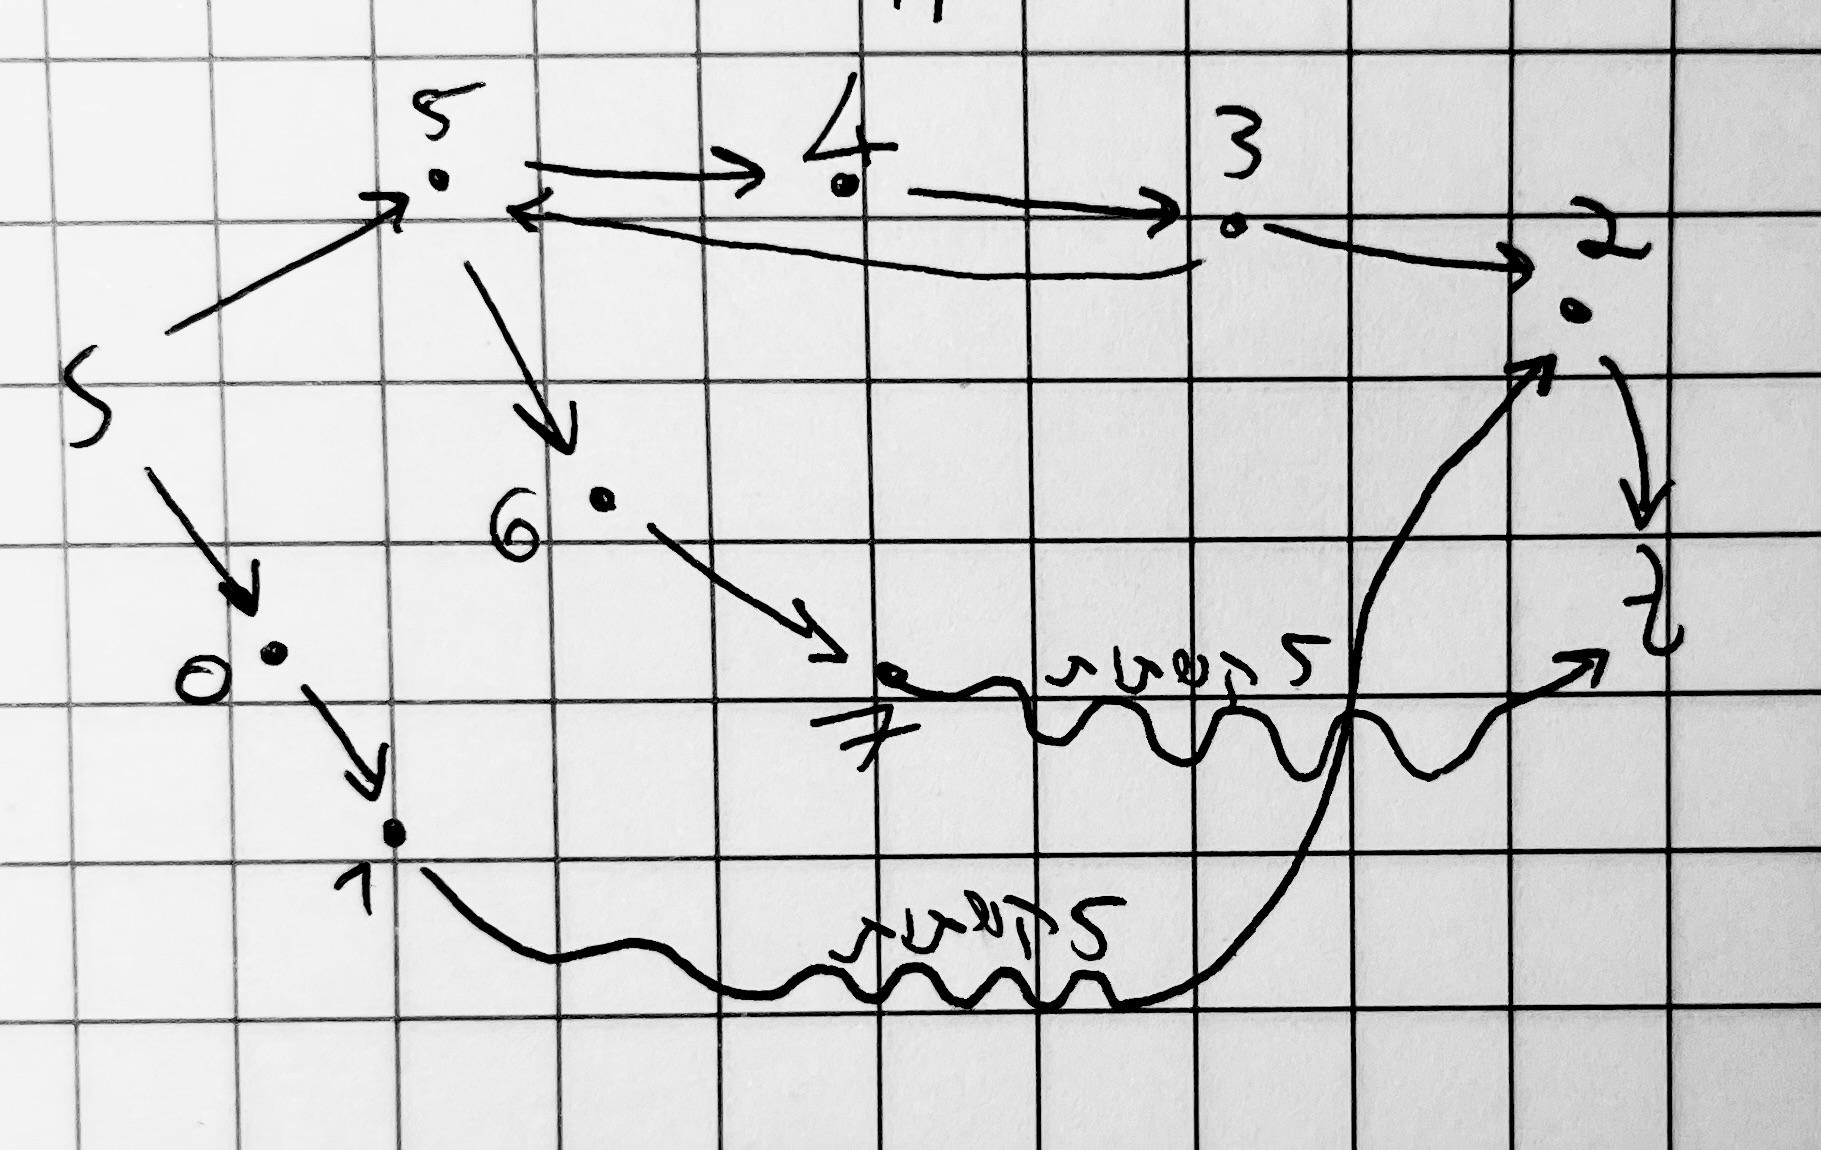
\includegraphics[width=0.3\linewidth]{2c/graph1.jpeg}
				\caption{גרף ההתחלה}
				\label{fig:graph1}
			\end{figure}
		\end{center}
		עבור קיבולים שלמים עם ערך $1$ (המסלול המקוקו הוא מסלול של 5 קשתות משורשרות). נבחין שהמק''ב הוא המסלול $s \to 5 \to 4 \to 3 \to 2 \to t$, ולאחריו הגרף השיורי יהיה: 
	\begin{center}
		\begin{figure}[h]
			\centering
			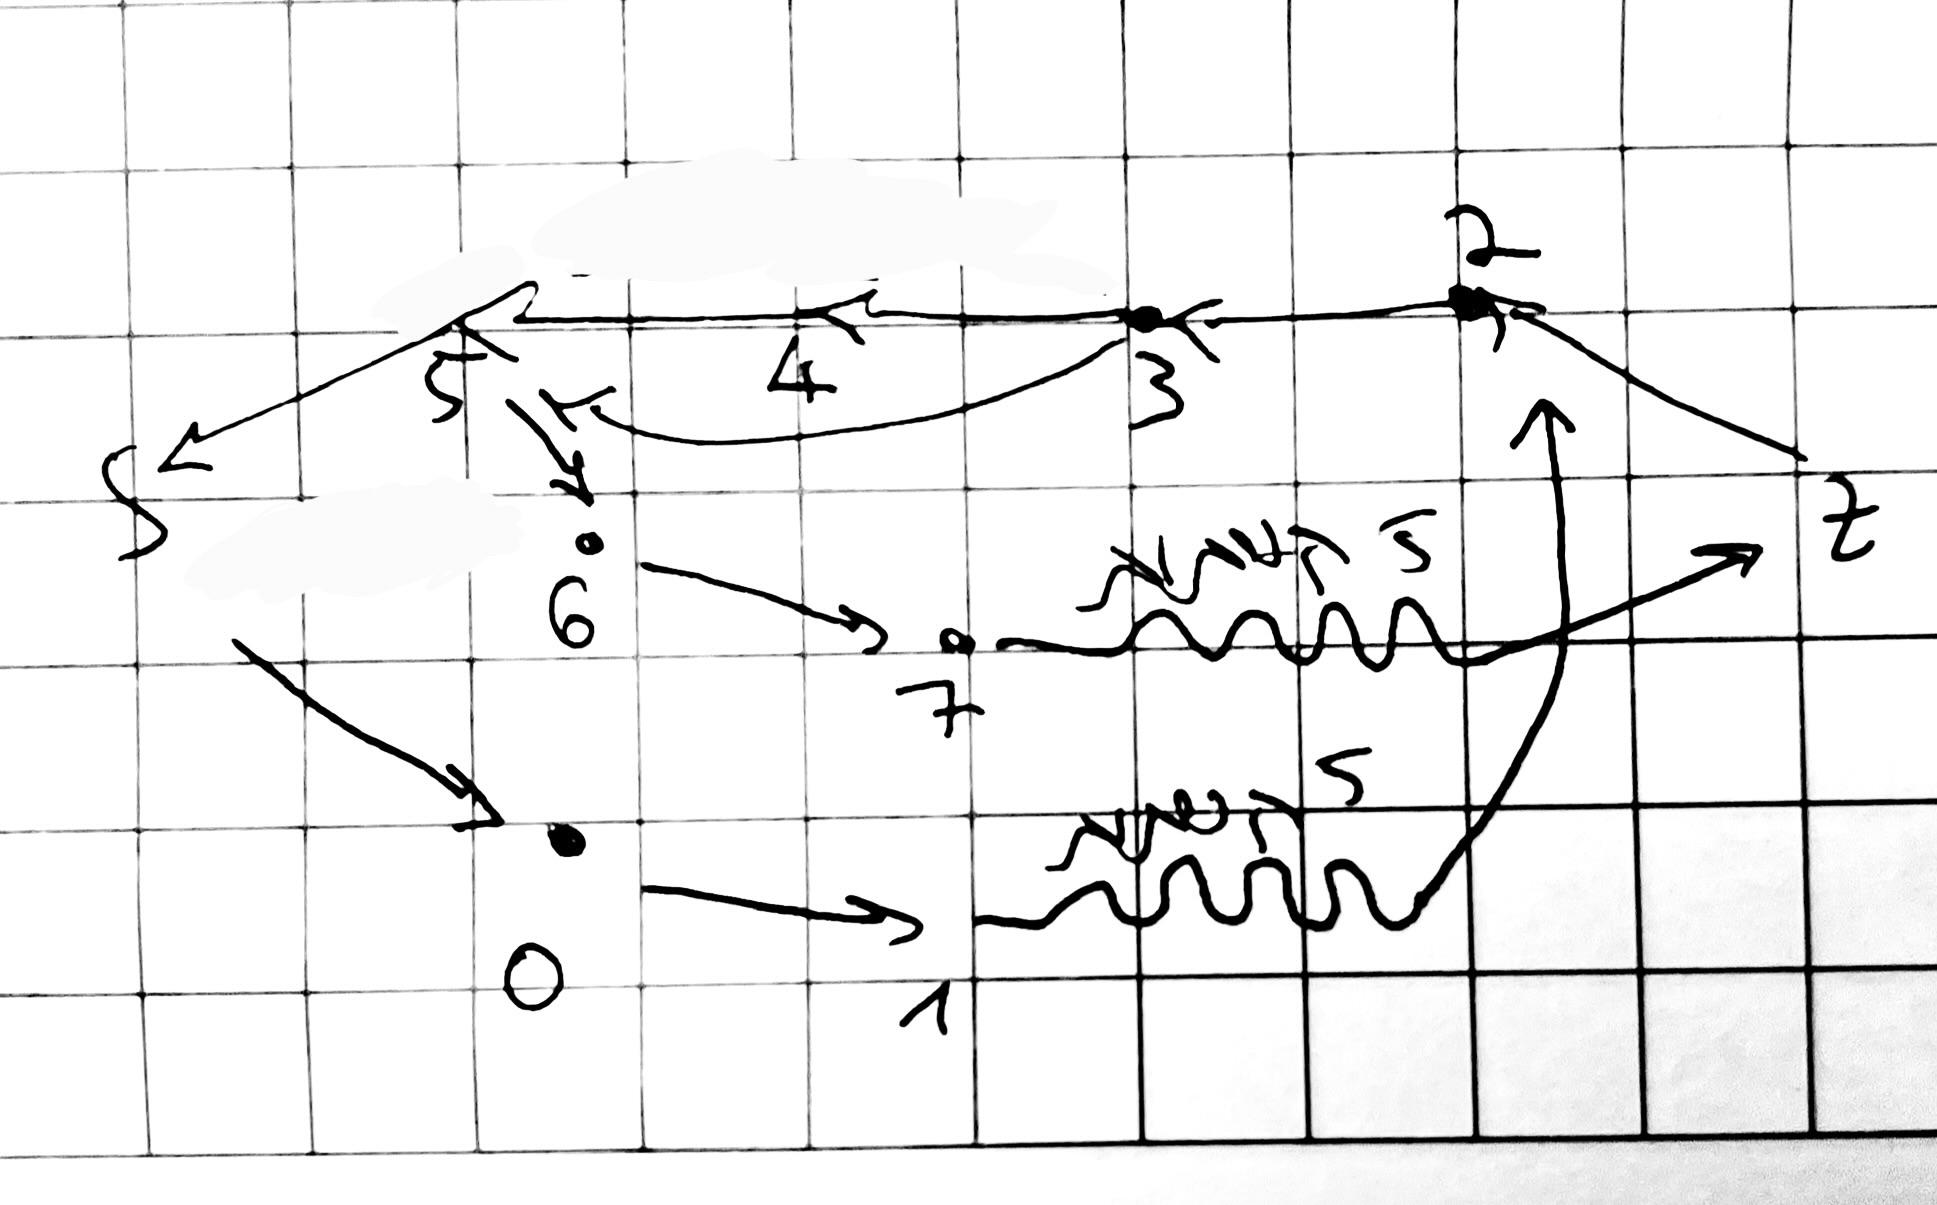
\includegraphics[width=0.3\linewidth]{2c/graph2.jpeg}
			\caption{הגרף השיורי $G_f$ לאחר הוספת המק''ב}
			\label{fig:graph2}
		\end{figure}
	\end{center}
	(טכנית הקיבול על $7 \to s$ הוא $2$ אבל זה לא משנה). נבחין שבו המק''ב הוא 
	\[ s \to 0 \to 1 \squig 2 \to 3 \to 4 \to 5 \to 6 \to 7 \squig t \]
	ובסיום הריצה קיבלנו מעגל $3 \to 4 \to 5 \to 3$ עם זרימה חיובית. 
		
		\item נתבונן בגרף $E = \{(s, t), (s, a), (a, t)\}$ עם קיבול $c \equiv 1$. עבור: 
		\[ f(e) = \begin{cases}
			0 & e = (s, a) \lor e = (a, t) \\
			1 & e = (s, t)
		\end{cases} \]
		וזרימה $h$ שמזרימה $1$ על כל הקשתות ב־$G_f$ (ולכן חוסמת בהכרח). נבחין שהגרף השיורי של $f + h$ כולל את המסלול $s \to t$ באורך $1$ בעוד בגרף השיורי של $G_f$ המקורי המק''ב הוא $s \to a \to t$, באורך $2$. לכן המרחקים קטנו בסתירה. 
%		\item נניח ש־$G = (V, E, c, s, t)$ רשת 01 (כלומר $\Img c = \{0, 1\}$) ונתונה זרימה $f \co E \to \{0, 1\}$. נמצא זרימה $f'$ בלי מעגלים. 
%		\begin{itemize}
%			\item \textbf{אלגוריתם: }נמצא מעגלים בעזרת DFS (כמו שראינו בהרצאה) ב־$G$. נסיר אותם, ונמשיך בלולאה עד ש־DFS לא מוצא יותר מעגלים (כלומר קשתות אחוריות) ב־$G$. לבסוף, נחזיר זרימה שמחזירה $1$ אמ''מ זו קשת ששרדה את ההסרות מ־$G$, אחרת $0$. בעיקר נותר להראות ש־$f'$ הסופית זרימה. בבירור $\Img f' \in \{0, 1\}$.
%			נוודא שהזרימה שיוצאת ונכנסת לכל קודקוד נשארת זהה, באינדוקציה על האיטרציה של הלולאה: יהי $v \in V$. מה.א. בלולאה הקודמת $f'$ הייתה זרימה, ומכאן שהזרם שנכנס ויצא מ־$v$ היה זהה. לאחר האיטרציה, אם $v$ לא על מעגל שהוסר, אין בעיה. אחרת נכנס זרם אחד פחות ויצא זרם אחד פחות (כי היא על מעגל $u \to v \to w \squig u$, ולכן $f(u, v) = f(v, w) = 0$ עתה)
%			\item \textbf{נכונות: }בבירור $f$ ללא מעגלים חיוביים, שכן $G$ באיטרציה הסופית ללא מעגלים מנכונות DFS. 
%			\item \textbf{סיבוכיות: }יש מעגלים לכל היותר כמספר הקשתות האחוריות, שחסום ב־$\sof E$. משום שהרצת DFS אורכת $\oc(\sof E + \sof V)$
%			סה''כ $\oc(\sof E \cdot (\sof E + \sof V))$. 
%		\end{itemize}
	\end{enumerate}
	
	\newpage \ \newpage 
%	\npage
%	\section{}
	\begin{enumerate}[(A)]
		\item נבדוק האם $e\str$
		\begin{itemize}
			\item \textbf{אלגוריתם: }נריץ דיניץ פעם אחת למציאת זרימה ממשקל $f$ (ב־$G$, ''הגרף המקורי``). נחסיר את קיבול $e\str$ (לקבלת ''הגרף השני``) ב־$1$ ונריץ דיניץ פעם שנייה על הגרף שקיבלנו לקבלתם זרימה $f'$. נחזיר תשובה חיובית אמ''מ $\sof f = \sof {f'} + 1$. 
			\item \textbf{נכונות: }נבחין שבהכרח $\sof {f'} \le \sof f$ (כי רק הקטנו קיבולים). עוד נבחין כי כל אחת מהזרימות משרה חתך מינימום מאותו הערך ממשפט MFMC. לכן בהכרח משקל חתכים מינימלים בגרף המקורי הוא $\sof f$. 
			\begin{itemize}
				\item[$\implies$]נניח ש־$e\str$ חוצה חתך מינימום כלשהו. אז בפרט אותו החתך יהיה מקיבול $\sof f - 1$ בגרף השני (נסכום את כל הקיבולים, כולל זה של $e\str$ שקטן ב־$1$) וסה''כ $\sof{f'} = \sof f - 1$ מ־MFMC. 
				\item[$\impliedby$]נניח ש־$\sof {f'} = \sof f - 1$. אז אם יש חתך מינימלי בגרף השני מקיבול $\sof f - 1$, בהכרח הוא גם חתך מינימלי בגרף המקורי (שכן $\sof{f'} \le \sof f$) מאותו הקיבול (אם בשלילה $e\str$) לא עליו. וזו סתירה כי אז $\sof f = \sof f - 1$ כלומר $0 = 1$. 
			\end{itemize}
			\item \textbf{סיבוכיות: }$\oc(\sof V^2 \sof E)$ של הרצת דיניץ פעמיים. 
		\end{itemize}
		\item נבדוק האם $e\str$ חוצה כל חתך מינימום בגרף. 
		\begin{itemize}
			\item \textbf{אלגוריתם: }נריץ דיניץ למציאת זרימה מקסימלית $f$ (ב־$G$, ''הגרף המקורי``). נעלה ב־$1$ את קיבול $e\str$ (לקבלת ''הגרף השני``) ונפעיל את דיניץ למציאת זרימה מקסימלית $f'$. נחזיר תשובה חיובית אמ''מ $\sof f + 1= \sof {f'}$. 
			\item \textbf{נכונות: }נבחין שבהכרח $\sof {f'} \ge \sof f$ (כי רק הגדלנו קיבולים). עוד נבחין כי כל אחת מהזרימות משרה חתך מינימום מאותו הערך ממשפט MFMC. לכן בהכרח משקל חתכים מינימלים בגרף המקורי הוא $\sof f$. 
			\begin{itemize}
				\item[$\implies$] נניח ש־$e\str$ חוצה כל חתך מינימום בגרף. בפרט כל חתך מינימום הוא מקיבול $\sof f + 1$. נבחין שבהכרח $e\str$ על החתך השני, שכן אם לא כך אז מדובר בחתך בגרף המקורי (כי הוא לא נוגע ב־$e\str$) ומשום ש־$\sof{f'} \ge \sof f$ מדובר בחתך מינימום גם בגרף המקורי, למרות ש־$e\str$ לא נמצאת עליו וזו סתירה. 
				\item[$\impliedby$] אם $\sof f + 1 = \sof{f'}$ למרות ש(בשלילה) ישנו חתך $(S, T)$ בגרף המקורי שלא כולל את $e\str$. אז זהו גם חתך בגרף השני מאותו הקיבול (שכן $e\str$ לא עליו) וזו סתירה למינימליות של $\sof{f'}$ (כי מצאנו חתך מקיבול $\sof f$ במקום $\sof f + 1$). 
			\end{itemize}
			סה''כ בשני הכיוונים הוכחנו נכונות. 
			\item \textbf{סיבוכיות: }$\oc(\sof V^2 \sof E)$ של הרצת דיניץ פעמיים. 
		\end{itemize}
	\end{enumerate}
	
	\newpage \ \newpage 
%	\npage
%	\section{}
	אינני יודע
	
	\newpage \ \newpage 
%	\npage
%	\section{}
	נתונים $m$ מכונות ו־$n$ משימות. לכל משימה $i \in [n]$ נתון $L_i \subset [m]$ של מכונות שיודעות לבצע אותו. נגדיר $N = \sum_{i \in [n]} \sof{L_i}$ ונגדיר $W = \max\{W_j\}_{j \in [m]}$ כאשר $W_j$ מספר המשימות שהמכונה ה־$m$ יודעת לבצע. 
	\begin{itemize}
		\item \textbf{אלגוריתם: }ניצור $n$ צמתים $v_1 \dots v_n$ ל־$n$ משימות, ו־$m$ מכונות $u_1 \dots u_m$. נחבר את $s$ ל־$v_i$־ים ואת ה־$u_i$־ים ל־$t$. נוסיף קשת מכוונת $(v_i, u_j)$ אמ''מ $j \in L_i$ (כלומר המכונה ה־$j$ יודעת לבצע את המשימה ה־$i$). נגדיר $c \equiv 1$ קבוע, ונפעל באופן הבא: ראשית, נריץ את FF, אם $\sof f = n$ נחזיר התאמה חח''ע בין משימות למכונות, היא בהכרח מינימלית וסיימנו. אחרת, נעלה את הקיבולים של הקשתות $u_i \to t$ ב־$1$, ונריץ את FF על הזרימה הקודמת, נסיים גם כאן אם $\sof f = n$. נמשיך כך כשבכל איטציה FF מתחיל את הזרימה ההתחלתית שלו להיות הזרימה הקודמת. 
		\item \textbf{נכונות: }ישירות מהנכונות של השיוך של משימות למכונות מהתרגול. באיטרציה הראשונה נטפל במקרה ש־$W = 1$, אח''כ במקרה בו $W = 2$, וכו' עד שנגיע למקרה המקסימלי בו $W = n$. אם גם בו לא נמצא זרימה מתאימה בהכרח לא קיימת חלוקה של משימות למכונות. 
		\item \textbf{סיבוכיות: }האיטאציה הראשונה של FF תיארך $\oc(E \cdot {\sof f})$ בעוד הזרימה המקסימלית בגודל $n$ ו־$n + m + N = \sof E$, ולכן סה''כ $\oc(n(n + N + m))$. 
		
		אחרי האיטרציה הראשונה, במקרה הגרוע ניאלץ לבצע את כל $n$ האיטרציות. במקרה הזה כל המשימות יתנקזו למכונה אחת, ונידרש לבצע רק איטרציה אחת של FF שתמצא מסלול $s \squig t$. 
		
		סה''כ סיבוכיות $\oc(n \cdot (n + N + m))$. 
	\end{itemize}
	
	\newpage \ \newpage 
%	\npage
%	\section{}
	תהא $B \in \R^{n \times n}$ מטריצה חיובית שחוסמת מלמעלה pointwise מטריצה $M$. נניח שסכום איברי כל שורה חסום ב־$r_i$ וסכום איברי כל טור חסום ב־$c_i$. נמצא $M$ מקסימלית (ביחס ל־$\sof M \cod \sum_{i = 1}^{n}\sum_{j = 1}^{n}a_{ij}$). 
	\begin{itemize}
		\item \textbf{אלגוריתם: }נגדיר קודקודים $\tl r_1 \dots \tl r_n, \tl c_1 \dots \tl c_n$ ו־$s, t$ עם קשתות $(s, \tl r_i)$ בעלות קיבול $r_i$ ו־$(t, \tl c_i)$ עם קיבול $c_i$. נגדיר קשתות $(\tl r_i, \tl c_j)$ עם קיבול $b_{ij}$, ונמצא זרימה מקסימלית. נחזיר את $m_{ij} \cod f(\tl r_i, \tl c_i)$. 
		\item \textbf{נכונות: }נוכיח $M$ עומדת בתנאים ומקסימלית אמ''מ $M$ זרימה מקסימלית. 
		\begin{itemize}
			\item[$\implies$]נניח ש־$M$ עומדת בתנאים. הזרימה $f(\tl r_i, \tl c_i) = m_{ij}$ וכן $f(s, \tl r_i) = \sum_{j = 1}^{n}m_{ij} = \sum_{j = 1}^{n}f(\tl r_i, \tl c_j)$ ו־$f(\tl r_i, t) = \sum_{j = 1}^{n}m_{ji}$. קל לראות ש־$\sof f = \sof M$ (שכן $\sof f = \sum f(\tl r_i, t) = \sof M$ מהגדרה) ומשום ש־$f$ זרימה תקינה (בבירור מקיימת את אילוץ הקיבול) היא בהכרח מקסימלית (כי מצאנו התאמה חח''ע בין $M$ שעומדת בתנאים לבין זרימה תקינה, ו־$\sof f = M$). 
			\item[$\impliedby$]נניח שקיבלנו זרימה מקסימלית. אז נוכל לבנות מטריצה $m_{ij} = f(\tl r_i, \tl c_j)$. היא בבירור עומדת בתנאים שכן מאילוץ הקיבול על $(\tl r_i, \tl c_j)$ מתקיים ש־$m_{ij} = f(\tl r_i, \tl c_j) \le c(\tl r_i, \tl c_j) = b_{ij}$ ומאילוץ הקיבול על $(s, \tl r_i)$ נקבל מצד אחד ש־$\sum_{j = 1}^{n}m_{ij} = \sum_{j = 1}^{n} f(\tl r_i, \tl c_j) \le f(s, \tl r_i)$ (אחרת אין מספיק זרם להזרים) ומצד שני ש־$f(s, \tl r_i) \le r_i$ (מאילוץ הקיבול) ולכן $\sum_{j = 1}^{n}m_{ij} \le r_i$ כנדרש. באופן דומה על $c_i$. המקסימליות גם כן באופן דומה לצד השני של הגרירה (על בסיס כך ש־$\sof f = M$). 
		\end{itemize}
		\item \textbf{סיבוכיות: }מדובר על גרף עם $n^{2} + 2n = \sof E$ ו־$\sof V = 2n + 2$. מכיוון שהגרף דו''צ נגיע לסיבוכיות של $\oc(n^{2}\sqrt n)$. 
	\end{itemize}
	
	\newpage \ \newpage 
%	\npage
%	\section{}
	נתונה רשת זרימה $G = (V, E, c, s, t)$ וזרימת מקסימום $f$. נמצא אלגוריתם יעיל שבודק האם קיימים ברשת שני חתכים שונים שכל אחד מהם הוא מינימלי. 
	\begin{itemize}
		\item \textbf{אלגוריתם: }נמצא חתך מינימלי ב־$G$ לפי האלגוריתם מהתרגול. נחשב את $G^{T}$
		 וגם בו נמצא חתך מינימלי (רק שנחליף בין $s$ ל־$t$, כלומר נמצא זרימת מקסימום ב־$(V, E^T, c^T, t, s)$ כאשר $c^T(u, v) = c(v, u)$ ו־$E^T$ מוגדר בהתאם להרצאה), רק שהפעם נשתמש בזרימה $f^{T}(u, v) = f(v, u)$. נחזיר תשובה חיובית אמ''מ שני החתכים זהים. 
		\item \textbf{נכונות: }כדי להראות שהאלגו' מהתרגול בפעם השנייה יחזיר חתך תקין יש להראות ש־$f^{T}$ זרימת מקסימום בגרף המשוחלף. אנטי־סימטריות הינה מיידית, ואכן מתקיים אילוץ הקיבול שכן $f^{T}(v, u) \le c^{T}(v, u)$ ב־$G^{T}$ אמ''מ $f(u, v) \le c(u, v)$ ב־$G$ (ישירות מההגדרה $f(v, u) = f^{T}(u, v)$ ו־$c(v, u) = c^{T}(u, v)$). 
		
		עתה אנו מחזיקים בשני חתכים, $(S_1, T_1)$ ב־$G$ ו־$(S_2, T_2)$ ב־$G^{T}$, כל אחד חתך מינימום. 
		מכיוון אחד, אם $(S_1, T_1) \neq (S_2, T_2)$ אז בבירור $(S_2, T_2)$ גם חתך מינימום ב־$G$ ולכן מצאנו את הנדרש. אחרת, נניח בשלילה שהם זהים אך יש חתך $(S_0, T_0)$ אחר ששונה להם. אז קיים $v \in S \cap T_1 = S \cap T_2$. ע''פ האלגוריתם, $v$ לא נגיש (ע''י BFS) מ־$s$ ב־$G_f$ אך $v$ נגיש מ־$t$ ב־$G^T_{f^T}$ (הגרפים השיוריים). לכן מהגדרת רשת הזרימה המשוחלפת $v$ נגיש מ־$s$ ב־$G_f$, וזו סתירה. 
	\end{itemize}
	
	\newpage \ \newpage 
%	\npage
%	\section{}
	החלטתי לפרוש מחיי האקדמיה בשיא ולנסות להפיק סרט. $A = \{a_1 \dots a_n\}$ רשימת השחקנים, כאשר $a_i$ דורש משכורת של $p_i$. $B = \{b_1 \dots b_m\}$ רשימת המשקיעים, כאשר $b_j$ מוכן להשקיע $q_j$, בתנאי שהשחקנים האהובים עליו $A_j \subset A$ ישחקו בסרט. 
	
	נמצא אלגוריתם שמוצא בחירת שחקנים ומשקיעים עם רווח הפקה מירבי. 
	
	\begin{itemize}
		\item \textbf{אלגוריתם: }נגדיר $V = A \cup B \cup \{s, t\}$. נשלח קשתות מ־$s$ לאיברי $B$ (המשקיעים) מהצורה $(s, b_i)$ עם קיבול $c(s, b_i) = q_i$. מ־$A$ (השחקנים) ל־$t$ נשלח קשתות $(a_i, t)$ עם קיבול $c(a_i, t) = p_i$. נוסיף קשת $(b_j, a_i)$ אמ''מ $a_i \in A_j$ עם קיבול אינסופי (נוכל להעביר כמה זרימה שנרצה. זה לא משפיע מהותית על האלגוריתם, רק צריך לוודא שהבעיה חסומה). 
		
		נמצא באמצעות דיניץ זרימה מקסימלית, ונשתמש באלגוריתם מהתרגול (שני BFS־ים על הגרף השיורי) למציאת חתך $(S, T)$ מינימלי מזרימה. נחזיר את השחקנים והמשקיעים שב־$S$. 
		\item \textbf{נכונות: }ראשית, נבחין שהבעיה לא חסומה, לדוגמה עבור חתך שחוצה את הקשתות מ־$s$ ל־$B$ (קיבולו $\sum q_i$ סופי, והוא שקול לבחירת אף אחד מהמשקיעים). עתה נוכיח שקילות. 
		\begin{itemize}
			\item[$\implies$] יהי חתך $(S, T)$ מינימלי. נוכיח שהוא משרה רווח הפקה מירבי. הוא  אכן משרה רווח הפקה תיקני כי הראנו שהבעיה חסומה, כלומר ניתן למצוא חתך שלא עובר דרך קשתות מקיבול אינסופי. לכן, אם $b_i \in S$ בהכרח גם כל קשת מהצורה $(b_i, a_j)$ ב־$S$, דהיינו $A_i \in S$ מהגדרת $E$ והקיבולים. יתרה מכך, נוכל להראות שהיא מינימלית. נסמן ב־$\Sg$ את הסכום $\sum_{i \in B}q_i$ (סך ההשקעות). 
			נבחין שקיבול חתך $(S, T)$ שבו \textbf{לא} בחרנו את המשקיעים $Q \subset B$ וכן בחרנו את השחקנים $P \subset A$ הוא: 
			\[ c(S, T) = \sum_{i \in Q}q_i + \sum_{j \in P}p_j = \Sg - \cl{\sum_{i \in Q}q_i - \sum_{j \in P}p_j} \]
			לכן $c(S, T)$ מינימלי אמ''מ $- \cl{\sum_{i \in Q}q_i - \sum_{j \in P}p_j}$ מינימלי (הם נבדלים בקבוע) אמ''מ $\sum_{i \in Q}q_i - \sum_{j \in P}p_j$ מקסימלי. אך נבחין שהביטוי האחרון הוא רווח ההפקה ולכן רווח ההפקה מקסימלי כאשר החתך מינימלי. 
			\item[$\impliedby$]תהא בחירה (עם רווח הפקה מקסימלי) של משקיעים ושחקנים, ונוכיח שהיא משרה חתך מינימלי. כבר הראנו (בבחירה הקודמת) שהחתך משרה קבוצת משקיעים עם רווח הפקה מקסימלי, ונבחין שהוא משרה מהגדרה את הקבוצה המקורית של משקיעים ושחקנים וסה''כ סיימנו. 
		\end{itemize}
		\item \textbf{סיבוכיות: }מדובר בגרף עם $\sof V = n + m$ ו־$\sof E = \sum \sof A_j \le nm$ ולכן סה''כ סיבוכיות דיניץ היא $\oc(\sof E \sqrt {\sof{V}}) = \oc\cl{nm\sqrt{n + m}}$. 
	\end{itemize}
	
	
%	\ndoc
\end{document}
